\documentclass{report}
\usepackage{graphicx} % Required for inserting images
\usepackage[italian]{babel}
\usepackage{tikz}
\usepackage{hyperref}
\usepackage{amsmath}
\usepackage{xcolor}
\usepackage{float}
\usepackage{soul}
\usepackage{listings} % Per evidenziare il codice

\definecolor{lightgray}{rgb}{0.9,0.9,0.9} % Definizione colore sfondo
\definecolor{darkgreen}{rgb}{0.0, 0.5, 0.0}

\lstset{
    backgroundcolor=\color{lightgray}, % Sfondo grigio
    basicstyle=\ttfamily, % Font monospaziato
    % frame=single, % Bordo attorno al codice
    tabsize=4, % Dimensione tabulazione
    breaklines=true, % Permette di andare a capo automaticamente
    numbers = left,
    numberstyle=\small\color{gray}
}

\title{\huge\textbf{{A.I. for Security}}}
\date{Parte II}

\begin{document}

\maketitle
\tableofcontents
\newpage

\chapter{GANs}

Prima dell'AI i controlli erano basati su signature, ovvero si facevano dei controlli tra l'hash dei miei programmi e quelli dei virus (noti).

\noindent Il polimorfismo dei virus ha ucciso questo metodo di controllo, dato che nel codice dei virus viene introdotto un fattore di casualità.

\noindent Per questa ragione è diventato fondamentale l'uso dell'intelligenza artificiale; nel modo tradizionale:
\begin{itemize}
    \item si raccolgono gli eventi generati dal malware per avere dei dati 
    \item viene fatto il training del modello con quei dati 
    \item quando un malware si comporterà in modo simile, il modello sarà in grado di dire \textit{"tu non sei esattamente quello ho visto, però sei 
    abbastanza simile! ti blocco!"}
\end{itemize}

\noindent $\rightarrow$ un attaccante mira ad attaccare sia la fase di training ed ancora di più a cercare di ingannare il modello in fase di inferenza

\section{Un nuovo paradigma: autoencoders}

Uno dei maggiori ostacoli per l'intelligenza artificiale quando si parla di sicurezza informatica, è la scarsita di dati a disposizione per fare 
il training dei modelli.

\noindent Una soluzione è quella di usare gli autoencoders per generare dei dati di training, allo scopo di ampliare il panorama statistico delle attività che un malware 
può fare; viene fatto per garantire al modello la capacità di generalizzare meglio, anche nel caso di input mai visti come gli \textit{0-day attacks}.

\newpage
\section{GANs}

Gli autoencoder sono un buon metodo per fare training, ma è meglio usare le GAN.

\noindent Un esempio di perché non è sufficiente usare gli autoencoder è che se vogliamo riconoscere il numero 7, se cambia un pixel viene
riconosciuto lo stesso come vero anche nel caso non lo sia, come nella figura.

\begin{figure}[H]
    \centering
    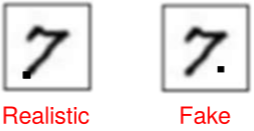
\includegraphics[width=0.4\linewidth]{images/seven.png}
\end{figure}

\noindent In associazione alle GANs si utilizza il discriminatore per rendere i dati generati indistinguibili da quelli reali.

\section{Il problema delle classi sbilanciate}

Supponiamo di avere migliaia di esempi di \textit{syscall} benigne, ma solo poche centinaia di esempi di \textit{syscall} generate 
da malware.

\noindent Se addestriamo un modello usando questo dataset sbilanciato, otteremo un classificatore che sarà anch'esso sbilanciato; magari otteniamo
un'accuratezza elevatissima sui dati di training, ma non devo esserne contento perché molto probabilmente il modello avrà imparato un 
predittore statico, incapace di generalizzare.

\noindent Uno strumento che viene in aiuto per capire se il modello sta imparando correttamente è la \textit{confusion matrix} (dove magari vediamo 
che abbiamo un'accuratezza dell 99\% perché viene sempre classificato come benigno); se quasi tutti gli elementi della classe minoritaria 
vengono classificati in modo errato, vuol dire che il modello sta imparando un predittore statico, e quindi avere un'accuratezza elevata 
non significa niente.

\noindent Questo avviene perché generalmente c'è un \textit{bias} verso la classe di maggioranza, dato che il modello mira a ridurre il tasso di 
errore globale senza prendere in considerazione fattori come le distribuzioni delle classi.

\newpage
\section{Alcune soluzioni all'apprendimento \\ sbilanciato}

\subsection{Undersampling}

Viene fatto un \textit{sampling} della classe maggioritaria (nel nostro dei malware, quella benigna), in modo da usare lo stesso numero 
di esempi maligni. Il training set viene così ribilanciato, ed anche se avrò meno conoscenza almeno il modello non imparerà uno 
stupido predittore statico.

\noindent Lo svantaggio di questa metodologia è quello di avere perdita di informazioni.

\subsection{Oversampling - SMOTE}

Viene usato un generatore per generare esempi ed evitare che le classi siano sbilanciate.

\noindent Lo svantaggio di questa metodologia è quello di causare overfitting nel modello, a causa di esempi generati troppo simili 
a quelli già esistenti 

\subsubsection{SMOTE}

\noindent SMOTE (\textit{Synthetic Minority Oversampling Technique}) è un metodo di oversampling che sintetizza nuovi esempi 
plausibili nella classe minoritaria; è importante perché oltre ad aumentare la dimensione del training set, ne aumenta anche la varietà.

La procedura per generare nuovi punti è la seguente:
\begin{itemize}
    \item per ogni punto della classe di minoranza, vengono presi i $k$ punti più vicini ad esso 
    \item tra i $k$ punti selezionati, vengono scelti in maniera casuali $j$ punti (con $j<k$)
    \item colleghiamo il punto originale con i punti $j$, ottenendo una sorta di stella 
    \item i punti vengono generate sulle linee che collegano il punto originale con i $j$
\end{itemize} 

$\Rightarrow$ con questo metodo si riesce ad aumentare sia la cardinalità senza diminuire la varianza

\begin{figure}[H]
    \centering
    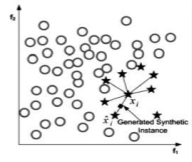
\includegraphics[width=0.5\linewidth]{images/smote.png}
\end{figure}

\noindent Tra gli svantaggi di SMOTE troviamo:
\begin{itemize}
    \item \textbf{\textit{Overgeneralization:}} potrebbe fare un \textit{oversample} di esempi rumorosi o che non sono informativi
    \item \textbf{\textit{Mancanza di flessibilità:}} il numero di punti sintetici generati deve essere fissato a priori, non permettendo 
    flessibilità in caso sia necessario un ri-bilanciamento
\end{itemize} 

\subsection{Cost-Sensitive approach}
Viene assegnato un peso a ciascun tipo di errore, in relazione a quale classe appartiene (maggioritaria o minoritaria); in questo posso ad esempio 
dare più peso alla classe che ha meno esempi ribilanciando il mio dataset a livello algoritmico (invece che a livello di dati).



\chapter{Federated Learning}

L'idea è quella di consentire il training collaborativo (nel senso di distribuito) di grandi modelli. Viene addestrato ciascun nodo della rete 
e poi ciò che viene mandato periodicamente ad un punto comune sono i parametri.

\noindent È un paradigma di estremo successo in tutti i quei casi dove è rilevante la privacy dell'utente, dato che non è necessario mandare 
i dati primari ma possono essere condivisi solamente i parametri.


\begin{figure}[H]
    \centering
    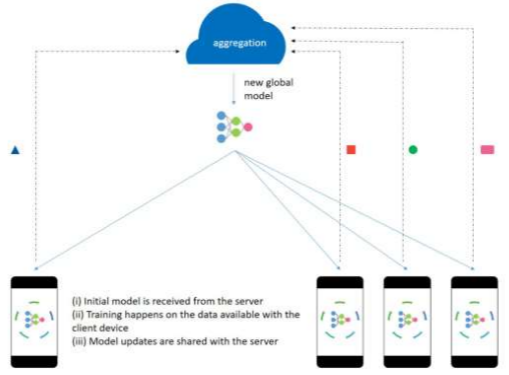
\includegraphics[width=0.8\linewidth]{images/fedrated-learning.png}
\end{figure}

\noindent Bisogna fare attenzione a dopo quanto tempo di training locale cominciare a condividere i parametri 
con il modello centrale.

\subsubsection{Possibile attacco}
Un attaccante potrebbe fare un attacco ai dati training, nel caso in risucisse ad aggiungersi ad un gruppo di nodi che condividono i loro 
parametri ad un modello federato.

\noindent Si può attaccare mandando dati casuali (\textbf{vandalismo}) o ancora peggio, si può attaccare mandando valori di pesi che cercano di 
far sì che poi il modello si comporti \textit{come voglio io} nel caso che mi interessa (\textbf{trojan horse}); è più facile fare un attacco 
rispetto al training classico centralizzato dove c'è un controllo dell'accesso.

\subsubsection{Considerazioni}

\begin{itemize}
    \item da un lato ho una garanzia di privacy, dato che i dati primari non vengono condivisi
    \item dall'altro è vulnerabile ad attacchi nella fase di training del modello 
\end{itemize}


\noindent Inoltre, ci possono essere problemi anche quando i partecipanti sono tutti onesti:
\begin{itemize}
    \item un partecipante smette di contribuire 
    \item un partecipante finisce i dati di addestramento 
    \item si fa fatica a fare un bilanciamento del modello centrale, dato che ogni nodo locale fa il suo bilanciamento locale 
    \item non so niente dei parametri che ricevo (magari è un predittore statico\dots)
\end{itemize}


\section{Sicurezza nel Federated Learning}

Quando si vuole fare un modello di minaccia la prima cosa da fare è un modello degli asset: per ogni asset si devono individuare i 
\textbf{failure mode}, ovvero modalità note con cui un asset può malfunionare.

\noindent Per sapere i failure mode di un modello di intelligenza artificiale, bisogna prendere delle proprietà generali desiderate (anche 
indipendenti dallo scenario, come 
ad esempio l'accuratezza); un failure mode è la negazione di una di queste proprietà.

\noindent Un esempio di due proprietà la cui negazione rappresenta un failure mode sono:
\begin{itemize}
    \item \textbf{Privacy:} avviene ad esempio quando qualcuno può ricostruire i valori del training set in sede di inferenza; nel caso del federated learning,
    si potrebbero avere problemi anche in sede di training, se un nodo perifico può dedurre i valori di training degli altri nodi 
    \item \textbf{Robustezza:} intesa come il numero di errori introdotti per ogni variazione del training set
\end{itemize}

\noindent Viene definito \textbf{threat} l'azione che porta ad un failure mode.

\noindent Un esempio di threat ad un modello di federated learning sono:
\begin{itemize}
    \item \textbf{\textit{Model Poisoning}}, iniettando dei pesi fasulli (vandalismo o trojan horse)
    \begin{itemize}
        \item potrei difendermi considerando come \textit{outlier} i valori che sono tre volte la deviazione standard (metodo del \textit{three-sigma}), 
        e facendo un filtraggio statistico (supponendo che siano una minoranza); ovviamente funziona solo su attacchi che mirano a modificare i valori 
        del training set per diminuire l'accuratezza complessiva del modello (vandalismo) e non attacchi avversariali, ovvero mirati a modificare un 
        un punto specifico del training set 
    \end{itemize}
    \item \textbf{\textit{Privacy Attack}}, cercando di trarre informazioni sugli altri modelli della rete; si dividono tra:
    \begin{itemize}
        \item \textit{\textbf{Reconstruction Attacks:}} mirano a ricostruire il training set originale e i dati degli utenti 
        \item \textbf{\textit{Membership Attacks:}} mirano a capire se un determinato dato specifico è presente nel training set
        \item $\Rightarrow$ potrei far viaggiare i pesi criptati, anche se comporta tutti i costi di avere un sistema di cifratura (criptare, decriptare, 
        gestione delle chiavi\dots); un'alternativa è quella di usare sistemi crittografici omomorifici, anche se hanno dei \textit{footprint}
        molto grossi rendendoli difficile da applicare in casi reali
    \end{itemize}
\end{itemize}

\noindent Una volta individuati i failure mode e i rispettivi threat, si può passare a fare un'analisi del rischio per cercare di limitare i possibili 
danni. Nel caso del federated learning abbiamo un rischio dovuto al fatto di avere un sistema distribuito invece che centralizzato.

















\end{document}